\documentclass[11pt,a4paper,]{article}
\usepackage{lmodern}

\usepackage{amssymb,amsmath}
\usepackage{ifxetex,ifluatex}
\usepackage{fixltx2e} % provides \textsubscript
\ifnum 0\ifxetex 1\fi\ifluatex 1\fi=0 % if pdftex
  \usepackage[T1]{fontenc}
  \usepackage[utf8]{inputenc}
\else % if luatex or xelatex
  \usepackage{unicode-math}
  \defaultfontfeatures{Ligatures=TeX,Scale=MatchLowercase}
\fi
% use upquote if available, for straight quotes in verbatim environments
\IfFileExists{upquote.sty}{\usepackage{upquote}}{}
% use microtype if available
\IfFileExists{microtype.sty}{%
\usepackage[]{microtype}
\UseMicrotypeSet[protrusion]{basicmath} % disable protrusion for tt fonts
}{}
\PassOptionsToPackage{hyphens}{url} % url is loaded by hyperref
\usepackage[unicode=true]{hyperref}
\hypersetup{
            pdftitle={Analysis of CO2 Emission and Energy Consumption around the world},
            pdfborder={0 0 0},
            breaklinks=true}
\urlstyle{same}  % don't use monospace font for urls
\usepackage{geometry}
\geometry{a4paper, centering, text={16cm,24cm}}
\usepackage[style=authoryear-comp,]{biblatex}
\addbibresource{references.bib}
\usepackage{color}
\usepackage{fancyvrb}
\newcommand{\VerbBar}{|}
\newcommand{\VERB}{\Verb[commandchars=\\\{\}]}
\DefineVerbatimEnvironment{Highlighting}{Verbatim}{commandchars=\\\{\}}
% Add ',fontsize=\small' for more characters per line
\usepackage{framed}
\definecolor{shadecolor}{RGB}{248,248,248}
\newenvironment{Shaded}{\begin{snugshade}}{\end{snugshade}}
\newcommand{\AlertTok}[1]{\textcolor[rgb]{0.94,0.16,0.16}{#1}}
\newcommand{\AnnotationTok}[1]{\textcolor[rgb]{0.56,0.35,0.01}{\textbf{\textit{#1}}}}
\newcommand{\AttributeTok}[1]{\textcolor[rgb]{0.77,0.63,0.00}{#1}}
\newcommand{\BaseNTok}[1]{\textcolor[rgb]{0.00,0.00,0.81}{#1}}
\newcommand{\BuiltInTok}[1]{#1}
\newcommand{\CharTok}[1]{\textcolor[rgb]{0.31,0.60,0.02}{#1}}
\newcommand{\CommentTok}[1]{\textcolor[rgb]{0.56,0.35,0.01}{\textit{#1}}}
\newcommand{\CommentVarTok}[1]{\textcolor[rgb]{0.56,0.35,0.01}{\textbf{\textit{#1}}}}
\newcommand{\ConstantTok}[1]{\textcolor[rgb]{0.00,0.00,0.00}{#1}}
\newcommand{\ControlFlowTok}[1]{\textcolor[rgb]{0.13,0.29,0.53}{\textbf{#1}}}
\newcommand{\DataTypeTok}[1]{\textcolor[rgb]{0.13,0.29,0.53}{#1}}
\newcommand{\DecValTok}[1]{\textcolor[rgb]{0.00,0.00,0.81}{#1}}
\newcommand{\DocumentationTok}[1]{\textcolor[rgb]{0.56,0.35,0.01}{\textbf{\textit{#1}}}}
\newcommand{\ErrorTok}[1]{\textcolor[rgb]{0.64,0.00,0.00}{\textbf{#1}}}
\newcommand{\ExtensionTok}[1]{#1}
\newcommand{\FloatTok}[1]{\textcolor[rgb]{0.00,0.00,0.81}{#1}}
\newcommand{\FunctionTok}[1]{\textcolor[rgb]{0.00,0.00,0.00}{#1}}
\newcommand{\ImportTok}[1]{#1}
\newcommand{\InformationTok}[1]{\textcolor[rgb]{0.56,0.35,0.01}{\textbf{\textit{#1}}}}
\newcommand{\KeywordTok}[1]{\textcolor[rgb]{0.13,0.29,0.53}{\textbf{#1}}}
\newcommand{\NormalTok}[1]{#1}
\newcommand{\OperatorTok}[1]{\textcolor[rgb]{0.81,0.36,0.00}{\textbf{#1}}}
\newcommand{\OtherTok}[1]{\textcolor[rgb]{0.56,0.35,0.01}{#1}}
\newcommand{\PreprocessorTok}[1]{\textcolor[rgb]{0.56,0.35,0.01}{\textit{#1}}}
\newcommand{\RegionMarkerTok}[1]{#1}
\newcommand{\SpecialCharTok}[1]{\textcolor[rgb]{0.00,0.00,0.00}{#1}}
\newcommand{\SpecialStringTok}[1]{\textcolor[rgb]{0.31,0.60,0.02}{#1}}
\newcommand{\StringTok}[1]{\textcolor[rgb]{0.31,0.60,0.02}{#1}}
\newcommand{\VariableTok}[1]{\textcolor[rgb]{0.00,0.00,0.00}{#1}}
\newcommand{\VerbatimStringTok}[1]{\textcolor[rgb]{0.31,0.60,0.02}{#1}}
\newcommand{\WarningTok}[1]{\textcolor[rgb]{0.56,0.35,0.01}{\textbf{\textit{#1}}}}
\usepackage{longtable,booktabs}
% Fix footnotes in tables (requires footnote package)
\IfFileExists{footnote.sty}{\usepackage{footnote}\makesavenoteenv{long table}}{}
\usepackage{graphicx,grffile}
\makeatletter
\def\maxwidth{\ifdim\Gin@nat@width>\linewidth\linewidth\else\Gin@nat@width\fi}
\def\maxheight{\ifdim\Gin@nat@height>\textheight\textheight\else\Gin@nat@height\fi}
\makeatother
% Scale images if necessary, so that they will not overflow the page
% margins by default, and it is still possible to overwrite the defaults
% using explicit options in \includegraphics[width, height, ...]{}
\setkeys{Gin}{width=\maxwidth,height=\maxheight,keepaspectratio}
\IfFileExists{parskip.sty}{%
\usepackage{parskip}
}{% else
\setlength{\parindent}{0pt}
\setlength{\parskip}{6pt plus 2pt minus 1pt}
}
\setlength{\emergencystretch}{3em}  % prevent overfull lines
\providecommand{\tightlist}{%
  \setlength{\itemsep}{0pt}\setlength{\parskip}{0pt}}
\setcounter{secnumdepth}{5}

% set default figure placement to htbp
\makeatletter
\def\fps@figure{htbp}
\makeatother


\title{Analysis of CO2 Emission and Energy Consumption around the world}

%% MONASH STUFF

%% CAPTIONS
\RequirePackage{caption}
\DeclareCaptionStyle{italic}[justification=centering]
 {labelfont={bf},textfont={it},labelsep=colon}
\captionsetup[figure]{style=italic,format=hang,singlelinecheck=true}
\captionsetup[table]{style=italic,format=hang,singlelinecheck=true}


%% FONT
\RequirePackage{bera}
\RequirePackage[charter,expert,sfscaled]{mathdesign}
\RequirePackage{fontawesome}

%% HEADERS AND FOOTERS
\RequirePackage{fancyhdr}
\pagestyle{fancy}
\rfoot{\Large\sffamily\raisebox{-0.1cm}{\textbf{\thepage}}}
\makeatletter
\lhead{\textsf{\expandafter{\@title}}}
\makeatother
\rhead{}
\cfoot{}
\setlength{\headheight}{15pt}
\renewcommand{\headrulewidth}{0.4pt}
\renewcommand{\footrulewidth}{0.4pt}
\fancypagestyle{plain}{%
\fancyhf{} % clear all header and footer fields
\fancyfoot[C]{\sffamily\thepage} % except the center
\renewcommand{\headrulewidth}{0pt}
\renewcommand{\footrulewidth}{0pt}}

%% MATHS
\RequirePackage{bm,amsmath}
\allowdisplaybreaks

%% GRAPHICS
\RequirePackage{graphicx}
\setcounter{topnumber}{2}
\setcounter{bottomnumber}{2}
\setcounter{totalnumber}{4}
\renewcommand{\topfraction}{0.85}
\renewcommand{\bottomfraction}{0.85}
\renewcommand{\textfraction}{0.15}
\renewcommand{\floatpagefraction}{0.8}


%\RequirePackage[section]{placeins}

%% SECTION TITLES


%% SECTION TITLES (NEW: Changing sections and subsections color)
\RequirePackage[compact,sf,bf]{titlesec}
\titleformat*{\section}{\Large\sf\bfseries\color[rgb]{0.8, 0.7, 0.1 }}
\titleformat*{\subsection}{\large\sf\bfseries\color[rgb]{0.8, 0.7, 0.1 }}
\titleformat*{\subsubsection}{\sf\bfseries\color[rgb]{0.8, 0.7, 0.1 }}
\titlespacing{\section}{0pt}{2ex}{.5ex}
\titlespacing{\subsection}{0pt}{1.5ex}{0ex}
\titlespacing{\subsubsection}{0pt}{.5ex}{0ex}


%% TITLE PAGE
\def\Date{\number\day}
\def\Month{\ifcase\month\or
 January\or February\or March\or April\or May\or June\or
 July\or August\or September\or October\or November\or December\fi}
\def\Year{\number\year}

%% LINE AND PAGE BREAKING
\sloppy
\clubpenalty = 10000
\widowpenalty = 10000
\brokenpenalty = 10000
\RequirePackage{microtype}

%% PARAGRAPH BREAKS
\setlength{\parskip}{1.4ex}
\setlength{\parindent}{0em}

%% HYPERLINKS
\RequirePackage{xcolor} % Needed for links
\definecolor{darkblue}{rgb}{0,0,.6}
\RequirePackage{url}

\makeatletter
\@ifpackageloaded{hyperref}{}{\RequirePackage{hyperref}}
\makeatother
\hypersetup{
     citecolor=0 0 0,
     breaklinks=true,
     bookmarksopen=true,
     bookmarksnumbered=true,
     linkcolor=darkblue,
     urlcolor=blue,
     citecolor=darkblue,
     colorlinks=true}

\usepackage[showonlyrefs]{mathtools}
\usepackage[no-weekday]{eukdate}

%% BIBLIOGRAPHY

\makeatletter
\@ifpackageloaded{biblatex}{}{\usepackage[style=authoryear-comp, backend=biber, natbib=true]{biblatex}}
\makeatother
\ExecuteBibliographyOptions{bibencoding=utf8,minnames=1,maxnames=3, maxbibnames=99,dashed=false,terseinits=true,giveninits=true,uniquename=false,uniquelist=false,doi=false, isbn=false,url=true,sortcites=false}

\DeclareFieldFormat{url}{\texttt{\url{#1}}}
\DeclareFieldFormat[article]{pages}{#1}
\DeclareFieldFormat[inproceedings]{pages}{\lowercase{pp.}#1}
\DeclareFieldFormat[incollection]{pages}{\lowercase{pp.}#1}
\DeclareFieldFormat[article]{volume}{\mkbibbold{#1}}
\DeclareFieldFormat[article]{number}{\mkbibparens{#1}}
\DeclareFieldFormat[article]{title}{\MakeCapital{#1}}
\DeclareFieldFormat[article]{url}{}
%\DeclareFieldFormat[book]{url}{}
%\DeclareFieldFormat[inbook]{url}{}
%\DeclareFieldFormat[incollection]{url}{}
%\DeclareFieldFormat[inproceedings]{url}{}
\DeclareFieldFormat[inproceedings]{title}{#1}
\DeclareFieldFormat{shorthandwidth}{#1}
%\DeclareFieldFormat{extrayear}{}
% No dot before number of articles
\usepackage{xpatch}
\xpatchbibmacro{volume+number+eid}{\setunit*{\adddot}}{}{}{}
% Remove In: for an article.
\renewbibmacro{in:}{%
  \ifentrytype{article}{}{%
  \printtext{\bibstring{in}\intitlepunct}}}

\AtEveryBibitem{\clearfield{month}}
\AtEveryCitekey{\clearfield{month}}

\makeatletter
\DeclareDelimFormat[cbx@textcite]{nameyeardelim}{\addspace}
\makeatother

\author{\sf\Large\textbf{ Zhenyu Wu}\\ {\sf\large Master of Business Analytics\\[0.5cm]} \sf\Large\textbf{ Harsh Katiyar}\\ {\sf\large Master of Business Analytics\\[0.5cm]} \sf\Large\textbf{ Liwen Pan}\\ {\sf\large Master of Business Analytics\\[0.5cm]} \sf\Large\textbf{ Josephine Valensia}\\ {\sf\large Master of Business Analytics\\[0.5cm]}}

\date{\sf\Date~\Month~\Year}
\makeatletter
\lfoot{\sf Wu, Katiyar, Pan, Valensia: \@date}
\makeatother


%%%% PAGE STYLE FOR FRONT PAGE OF REPORTS

\makeatletter
\def\organization#1{\gdef\@organization{#1}}
\def\telephone#1{\gdef\@telephone{#1}}
\def\email#1{\gdef\@email{#1}}
\makeatother
  \organization{Monash University}

  \def\name{Department of Business and Econometrics}

  \telephone{(03) 9905 2478}

  \email{questions@company.com}                 %NEW: New email addresss

\def\webaddress{\url{http://company.com/stats/consulting/}} %NEW: URl
\def\abn{12 377 614 630}                                    % NEW: ABN
\def\logo{\includegraphics[width=6cm]{Figures/logo}}  %NEW: Changing logo
\def\extraspace{\vspace*{1.6cm}}
\makeatletter
\def\contactdetails{\faicon{phone} & \@telephone \\
                    \faicon{envelope} & \@email}
\makeatother

%%%% FRONT PAGE OF REPORTS

\def\reporttype{Report for}

\long\def\front#1#2#3{
\newpage
\begin{singlespacing}
\thispagestyle{empty}
\vspace*{-1.4cm}
\hspace*{-1.4cm}
\hbox to 16cm{
  \hbox to 6.5cm{\vbox to 14cm{\vbox to 25cm{
    \logo
    \vfill
    \parbox{6.3cm}{\raggedright
      \sf\color[rgb]{0.8, 0.7, 0.1 }    % NEW color 
      {\large\textbf{\name}}\par
      \vspace{.7cm}
      \tabcolsep=0.12cm\sf\small
      \begin{tabular}{@{}ll@{}}\contactdetails
      \end{tabular}
      \vspace*{0.3cm}\par
      ABN: \abn\par
    }
  }\vss}\hss}
  \hspace*{0.2cm}
  \hbox to 1cm{\vbox to 14cm{\rule{4pt}{26.8cm}\vss}\hss\hfill}  %NEW: Thicker line
  \hbox to 10cm{\vbox to 14cm{\vbox to 25cm{   
      \vspace*{3cm}\sf\raggedright
      \parbox{11cm}{\sf\raggedright\baselineskip=1.2cm
         \fontsize{24.88}{30}\color[rgb]{0, 0.29, 0.55}\sf\textbf{#1}}   % NEW: title color blue
      \par
      \vfill
      \large
      \vbox{\parskip=0.8cm #2}\par
      \vspace*{2cm}\par
      \reporttype\\[0.3cm]
      \hbox{#3}%\\[2cm]\
      \vspace*{1cm}
      {\large\sf\textbf{\Date~\Month~\Year}}
   }\vss}
  }}
\end{singlespacing}
\newpage
}

\makeatletter
\def\titlepage{\front{\expandafter{\@title}}{\@author}{\@organization}}
\makeatother

\usepackage{setspace}
\setstretch{1.5}

%% Any special functions or other packages can be loaded here.
\usepackage{booktabs}
\usepackage{longtable}
\usepackage{array}
\usepackage{multirow}
\usepackage{wrapfig}
\usepackage{float}
\usepackage{colortbl}
\usepackage{pdflscape}
\usepackage{tabu}
\usepackage{threeparttable}
\usepackage{threeparttablex}
\usepackage[normalem]{ulem}
\usepackage{makecell}
\usepackage{xcolor}


\begin{document}
\titlepage

\section*{Country China and USA}

\hypertarget{read-data}{%
\subsection{Read data}\label{read-data}}

\begin{Shaded}
\begin{Highlighting}[]
\FunctionTok{options}\NormalTok{(}\AttributeTok{scipen =} \DecValTok{200}\NormalTok{)}
\NormalTok{Analysis\_Data }\OtherTok{\textless{}{-}} \FunctionTok{read\_csv}\NormalTok{(here}\SpecialCharTok{::}\FunctionTok{here}\NormalTok{(}\StringTok{"Data/Assignment\_data.csv"}\NormalTok{))}
\end{Highlighting}
\end{Shaded}

\hypertarget{data-preprocessing}{%
\subsection{Data preprocessing}\label{data-preprocessing}}

\begin{Shaded}
\begin{Highlighting}[]
\CommentTok{\# filtering data from 1970 to 2017 for China and the United States}
\NormalTok{data }\OtherTok{\textless{}{-}}\NormalTok{ Analysis\_Data }\SpecialCharTok{\%\textgreater{}\%}
  \FunctionTok{filter}\NormalTok{(Entity }\SpecialCharTok{\%in\%} \FunctionTok{c}\NormalTok{(}\StringTok{"China"}\NormalTok{,}\StringTok{"United States"}\NormalTok{)) }\SpecialCharTok{\%\textgreater{}\%}
  \FunctionTok{filter}\NormalTok{(Year}\SpecialCharTok{\textgreater{}=}\DecValTok{1970} \SpecialCharTok{\&}\NormalTok{ Year}\SpecialCharTok{\textless{}=}\DecValTok{2017}\NormalTok{)}
\FunctionTok{dim}\NormalTok{(data)}
\end{Highlighting}
\end{Shaded}

\begin{verbatim}
## [1] 96  7
\end{verbatim}

\hypertarget{overall-descriptive-statistical-analysis}{%
\subsection{Overall descriptive statistical analysis}\label{overall-descriptive-statistical-analysis}}

\begin{Shaded}
\begin{Highlighting}[]
\NormalTok{data }\OtherTok{\textless{}{-}}\NormalTok{ data }\SpecialCharTok{\%\textgreater{}\%}
  \FunctionTok{rename}\NormalTok{(}\AttributeTok{Average.annual.hours.worked=}
        \StringTok{"Average annual hours worked by persons engaged (avh) (PWT 9.1 (2019))"}\NormalTok{,}
        \AttributeTok{GDP.per.capita=}\StringTok{"Output{-}side real GDP per capita (gdppc\_o) (PWT 9.1 (2019))"}\NormalTok{,}
        \AttributeTok{Population=}\StringTok{"Population (historical estimates)"}\NormalTok{,}
        \AttributeTok{Country=}\NormalTok{Entity) }
\NormalTok{ overall }\OtherTok{\textless{}{-}}\NormalTok{ data }\SpecialCharTok{\%\textgreater{}\%}
    \FunctionTok{group\_by}\NormalTok{(Country) }\SpecialCharTok{\%\textgreater{}\%}
    \FunctionTok{summarise\_at}\NormalTok{(}\FunctionTok{c}\NormalTok{(}\StringTok{"Average.annual.hours.worked"}\NormalTok{,}\StringTok{"GDP.per.capita"}\NormalTok{,}\StringTok{"Population"}\NormalTok{),}
                 \FunctionTok{list}\NormalTok{(}\AttributeTok{Minimum =} \SpecialCharTok{\textasciitilde{}}\FunctionTok{min}\NormalTok{(.,}\AttributeTok{na.rm=}\ConstantTok{TRUE}\NormalTok{), }
                      \AttributeTok{Median =} \SpecialCharTok{\textasciitilde{}}\FunctionTok{median}\NormalTok{(.,}\AttributeTok{na.rm=}\ConstantTok{TRUE}\NormalTok{), }
                      \AttributeTok{Mean =} \SpecialCharTok{\textasciitilde{}}\FunctionTok{mean}\NormalTok{(.,}\AttributeTok{na.rm=}\ConstantTok{TRUE}\NormalTok{),}
                      \AttributeTok{Maximum =} \SpecialCharTok{\textasciitilde{}}\FunctionTok{max}\NormalTok{(.,}\AttributeTok{na.rm=}\ConstantTok{TRUE}\NormalTok{))) }\SpecialCharTok{\%\textgreater{}\%}
    \FunctionTok{pivot\_longer}\NormalTok{(}\SpecialCharTok{!}\NormalTok{Country, }\AttributeTok{names\_sep =}\StringTok{"\_"}\NormalTok{,}
                 \AttributeTok{names\_to =} \FunctionTok{c}\NormalTok{(}\StringTok{"Variable"}\NormalTok{, }\StringTok{".value"}\NormalTok{))}\SpecialCharTok{\%\textgreater{}\%}
   \FunctionTok{mutate}\NormalTok{(}\AttributeTok{Variable=}\FunctionTok{ifelse}\NormalTok{(Variable}\SpecialCharTok{==}\StringTok{"Average.annual.hours.worked"}\NormalTok{,}
                          \StringTok{"Hours.worked"}\NormalTok{,Variable))}
\end{Highlighting}
\end{Shaded}

\begin{Shaded}
\begin{Highlighting}[]
\NormalTok{knitr}\SpecialCharTok{::}\FunctionTok{kable}\NormalTok{(overall, }\AttributeTok{digits =} \DecValTok{2}\NormalTok{,}
    \AttributeTok{caption =} \StringTok{"Descriptive statistical analysis of China and the United States"}\NormalTok{)}
\end{Highlighting}
\end{Shaded}

\begin{table}

\caption{\label{tab:Table1}Descriptive statistical analysis of China and the United States}
\centering
\begin{tabular}[t]{l|l|r|r|r|r}
\hline
Country & Variable & Minimum & Median & Mean & Maximum\\
\hline
China & Hours.worked & 1969.39 & 1985.48 & 2049.81 & 2192.35\\
\hline
China & GDP.per.capita & 1394.16 & 3127.29 & 4574.76 & 13042.65\\
\hline
China & Population & 827601385.00 & 1224418542.50 & 1179497606.85 & 1421021794.00\\
\hline
United States & Hours.worked & 1729.96 & 1795.14 & 1799.27 & 1891.41\\
\hline
United States & GDP.per.capita & 23285.58 & 37978.02 & 39046.42 & 54794.76\\
\hline
United States & Population & 209513340.00 & 260886667.00 & 264561185.08 & 325084758.00\\
\hline
\end{tabular}
\end{table}

\hypertarget{trends-in-average-annual-hours-worked-and-gdp-per-capita}{%
\subsection{Trends in average annual hours worked and GDP per capita}\label{trends-in-average-annual-hours-worked-and-gdp-per-capita}}

\begin{Shaded}
\begin{Highlighting}[]
\FunctionTok{ggplot}\NormalTok{(data,}\AttributeTok{mapping =} \FunctionTok{aes}\NormalTok{(}\AttributeTok{x =}\NormalTok{ Year,}\AttributeTok{y=}\NormalTok{GDP.per.capita,}
                           \AttributeTok{color=}\NormalTok{Country,}\AttributeTok{group=}\NormalTok{Country)) }\SpecialCharTok{+}
  \FunctionTok{geom\_line}\NormalTok{() }\SpecialCharTok{+}
  \FunctionTok{labs}\NormalTok{(}\AttributeTok{y =}\StringTok{"GDP per capita"}\NormalTok{, }
       \AttributeTok{caption =} \StringTok{"Source: World Bank data base"}\NormalTok{)}\SpecialCharTok{+}
    \FunctionTok{theme\_bw}\NormalTok{()}
\end{Highlighting}
\end{Shaded}

\begin{figure}
\centering
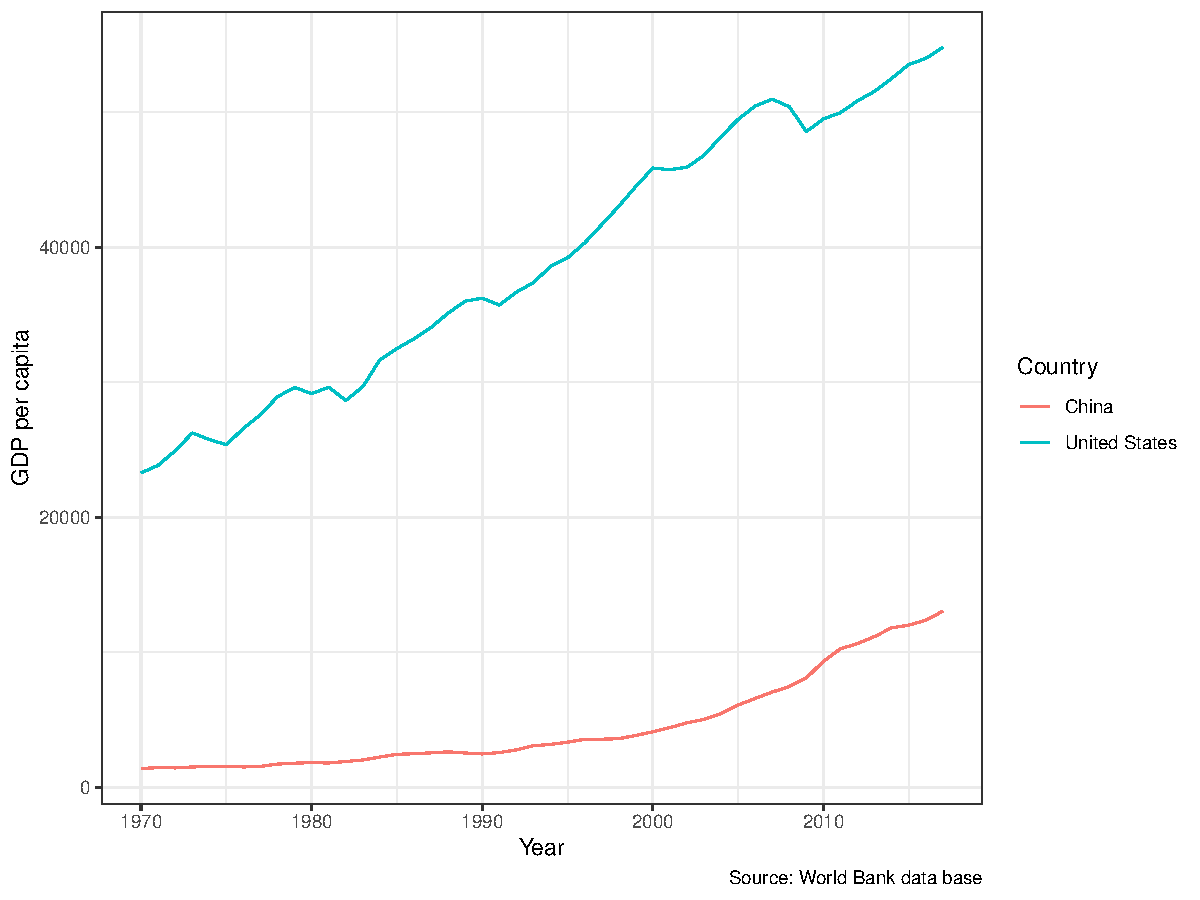
\includegraphics{report_files/figure-latex/Figure1-1.pdf}
\caption{\label{fig:Figure1}Trends in GDP per capita}
\end{figure}

\begin{Shaded}
\begin{Highlighting}[]
\FunctionTok{ggplot}\NormalTok{(data,}\AttributeTok{mapping =} \FunctionTok{aes}\NormalTok{(}\AttributeTok{x =}\NormalTok{ Year,}\AttributeTok{y=}\NormalTok{Average.annual.hours.worked,}
                           \AttributeTok{color=}\NormalTok{Country,}\AttributeTok{group=}\NormalTok{Country)) }\SpecialCharTok{+}
  \FunctionTok{geom\_line}\NormalTok{() }\SpecialCharTok{+}
  \FunctionTok{labs}\NormalTok{(}\AttributeTok{y =}\StringTok{"Average annual hours worked"}\NormalTok{, }
       \AttributeTok{caption =} \StringTok{"Source: World Bank data base"}\NormalTok{)}\SpecialCharTok{+}
    \FunctionTok{theme\_bw}\NormalTok{()}
\end{Highlighting}
\end{Shaded}

\begin{figure}
\centering
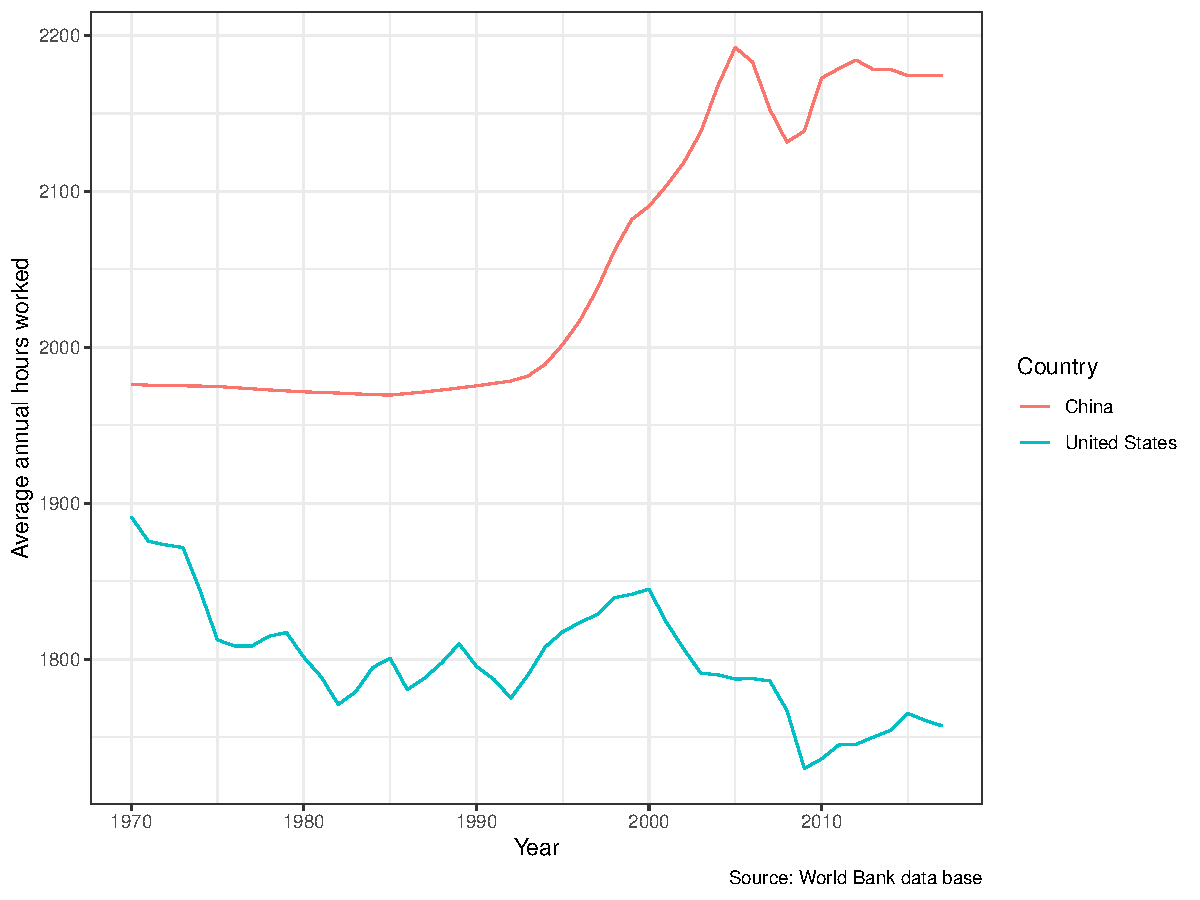
\includegraphics{report_files/figure-latex/Figure2-1.pdf}
\caption{\label{fig:Figure2}Trends in average annual hours worked}
\end{figure}

\hypertarget{the-relationship-between-average-annual-hours-worked-and-gdp}{%
\subsection{The relationship between average annual hours worked and GDP}\label{the-relationship-between-average-annual-hours-worked-and-gdp}}

\begin{Shaded}
\begin{Highlighting}[]
\NormalTok{data }\SpecialCharTok{\%\textgreater{}\%}
    \FunctionTok{filter}\NormalTok{(Country}\SpecialCharTok{==}\StringTok{"China"}\NormalTok{)}\SpecialCharTok{\%\textgreater{}\%}
    \FunctionTok{ggplot}\NormalTok{(}\AttributeTok{mapping =} \FunctionTok{aes}\NormalTok{(}\AttributeTok{x =}\NormalTok{ Average.annual.hours.worked,}
                          \AttributeTok{y=}\NormalTok{GDP.per.capita))}\SpecialCharTok{+}
    \FunctionTok{geom\_point}\NormalTok{() }\SpecialCharTok{+} 
    \FunctionTok{stat\_smooth}\NormalTok{(}\AttributeTok{method=}\NormalTok{lm)}\SpecialCharTok{+}
  \FunctionTok{labs}\NormalTok{(}\AttributeTok{x =}\StringTok{"Average annual hours worked"}\NormalTok{, }
       \AttributeTok{y =}\StringTok{"GDP per capita"}\NormalTok{, }
       \AttributeTok{caption =} \StringTok{"Source: World Bank data base"}\NormalTok{)}\SpecialCharTok{+}
    \FunctionTok{theme\_bw}\NormalTok{()}
\end{Highlighting}
\end{Shaded}

\begin{figure}
\centering
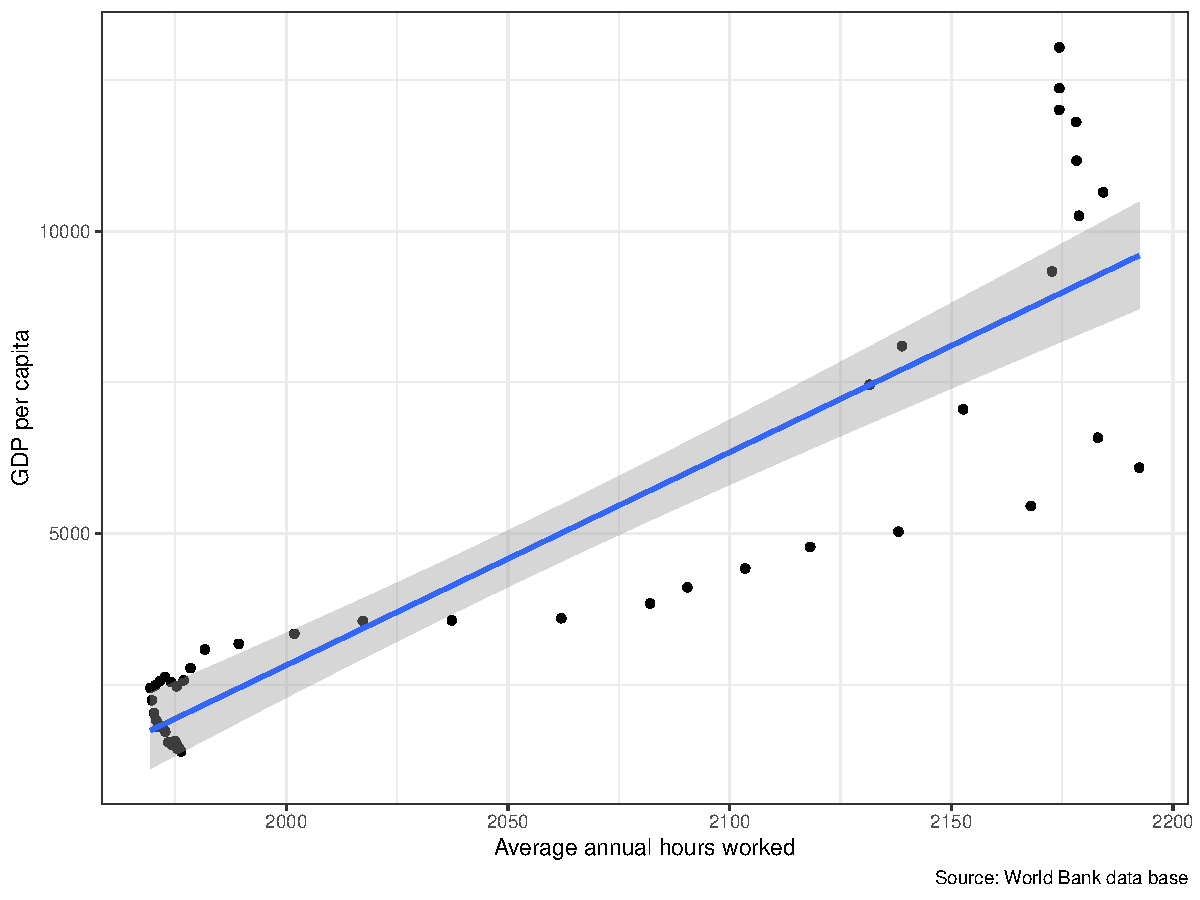
\includegraphics{report_files/figure-latex/Figure3-1.pdf}
\caption{\label{fig:Figure3}Relationship between average annual hours worked and GDP (China)}
\end{figure}

\begin{Shaded}
\begin{Highlighting}[]
\NormalTok{data }\SpecialCharTok{\%\textgreater{}\%}
    \FunctionTok{filter}\NormalTok{(Country}\SpecialCharTok{==}\StringTok{"United States"}\NormalTok{)}\SpecialCharTok{\%\textgreater{}\%}
    \FunctionTok{ggplot}\NormalTok{(}\AttributeTok{mapping =} \FunctionTok{aes}\NormalTok{(}\AttributeTok{x =}\NormalTok{ Average.annual.hours.worked,}
                          \AttributeTok{y=}\NormalTok{GDP.per.capita))}\SpecialCharTok{+}
    \FunctionTok{geom\_point}\NormalTok{() }\SpecialCharTok{+} 
    \FunctionTok{stat\_smooth}\NormalTok{(}\AttributeTok{method=}\NormalTok{lm)}\SpecialCharTok{+}
  \FunctionTok{labs}\NormalTok{(}\AttributeTok{x =}\StringTok{"Average annual hours worked"}\NormalTok{, }
       \AttributeTok{y =}\StringTok{"GDP per capita"}\NormalTok{, }
       \AttributeTok{caption =} \StringTok{"Source: World Bank data base"}\NormalTok{)}\SpecialCharTok{+}
    \FunctionTok{theme\_bw}\NormalTok{()}
\end{Highlighting}
\end{Shaded}

\begin{figure}
\centering
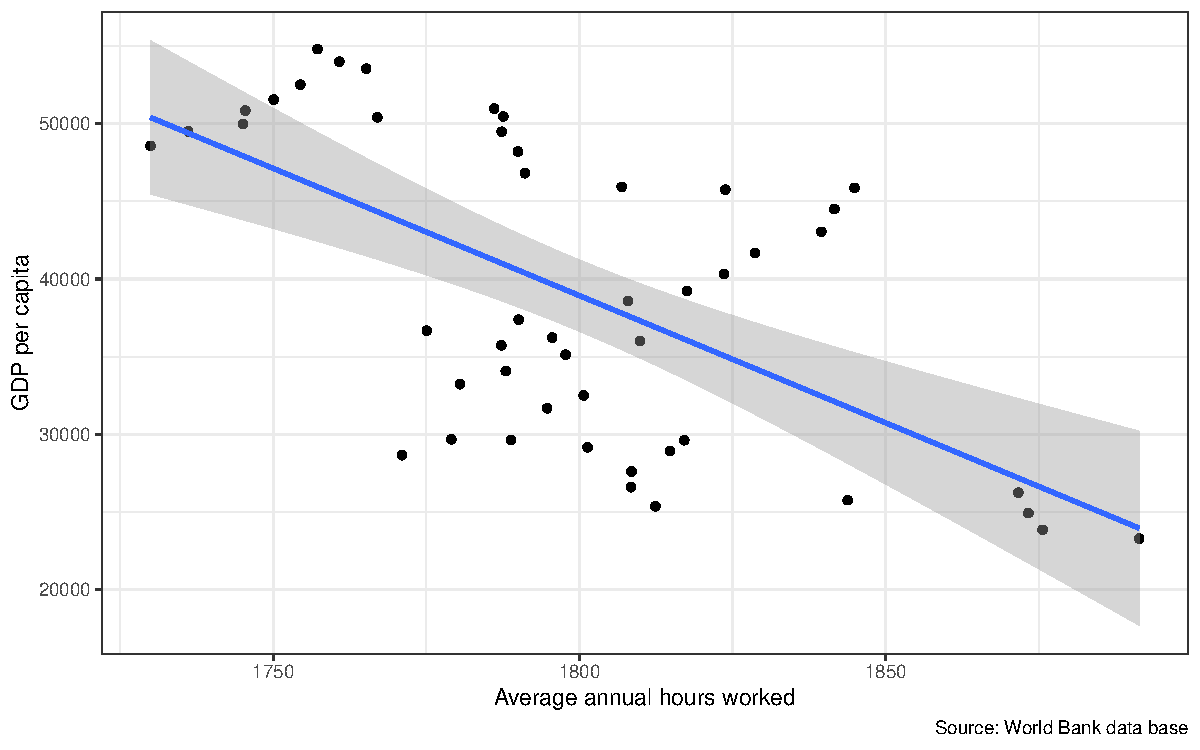
\includegraphics{report_files/figure-latex/Figure4-1.pdf}
\caption{\label{fig:Figure4}Relationship between average annual hours worked and GDP (United States)}
\end{figure}

\hypertarget{conclusion}{%
\subsection{Conclusion}\label{conclusion}}

In this section, I analyzed data from China and the United States. First, I filtered out the data for these two countries from 1970 to 2017. Then I performed an overall descriptive statistical analysis of the primary variables (Average.annual.hours.worked, GDP.per.capita and Population).

As shown in Table1\ref{tab:Table1}, the mean or median population in China is significantly larger than in the United States. But in GDP per capita, China is significantly less than the United States. And the average annual hours worked is slightly higher in China than in the United States.

The trends of GDP in China and USA in Figure\ref{fig:Figure1} shows that GDP per capita in both China and the U.S. is rising year by year, but the upward trend is more obvious in the United States. And for the average annual hours worked shown in Figure\ref{fig:Figure2}, I found a clear upward trend of average annual hours worked in China, while the United States has fluctuated but declined slightly overall.

Finally, I compared the relationship between average annual hours worked and GDP per capita in China and the United States. In China, the two variables showed a negative correlation in Figure\ref{fig:Figure3}, while in the United States of Figure\ref{fig:Figure4}, average annual hours worked decreases as GDP per capita rises.

\hypertarget{reference}{%
\subsection{Reference}\label{reference}}

{[}1{]} Wickham H, Averick M, Bryan J, et al.~Welcome to the Tidyverse{[}J{]}. Journal of open source software, 2019, 4(43): 1686.

{[}2{]} Wickham H, Chang W, Wickham M H. Package `ggplot2'{[}J{]}. Create elegant data visualisations using the grammar of graphics. Version, 2016, 2(1): 1-189.

\printbibliography

\end{document}
